%%%%%%%%%%%%%%%%%%%%%%%%%%%%%%%%%%%%%%%%%%%%%%%%%%%%%%%%%%%%%%%%%%%%%%%%%%%%%%%%
%2345678901234567890123456789012345678901234567890123456789012345678901234567890
%        1         2         3         4         5         6         7         8

\documentclass[letterpaper, 10 pt, conference]{ieeeconf}  % Comment this line out if you need a4paper

%\documentclass[a4paper, 10pt, conference]{ieeeconf}      % Use this line for a4 paper

\IEEEoverridecommandlockouts                              % This command is only needed if 
                                                          % you want to use the \thanks command

\overrideIEEEmargins                                      % Needed to meet printer requirements.

% See the \addtolength command later in the file to balance the column lengths
% on the last page of the document

% The following packages can be found on http:\\www.ctan.org
\usepackage{graphics} % for pdf, bitmapped graphics files
\usepackage{epsfig} % for postscript graphics files
\usepackage{mathptmx} % assumes new font selection scheme installed
\usepackage{times} % assumes new font selection scheme installed
\usepackage{amsmath} % assumes amsmath package installed
\usepackage{amssymb}  % assumes amsmath package installed
	
\title{\LARGE \bf
Structure of the set of feasible neural commands\\ for complex motor tasks
}

\author{Cohn BA$^{1}$, Szedl\'{a}k M$^{2}$, Fukuda K$^{2}$, Valero-Cuevas FJ$^{1}$, and  G{\"a}rtner B$^{2}$% <-this % stops a space
\thanks{*This work was supported by NIH NIAMS R01AR050520 and R01AR052345 grants, and SNF Project 200021-150055-1.
}% <-this % stops a space
\thanks{$^{1}$Departments of Biomedical Engineering and Computer Science at the University of Southern California Viterbi School of Engineering, Los Angeles, CA 90089, USA
        {\tt\small brianaco@usc.edu}}%
\thanks{$^{2}$Department of Computer Science, ETH Zurich, Switzerland}%
}


\begin{document}



\maketitle
\thispagestyle{empty}
\pagestyle{empty}


%%%%%%%%%%%%%%%%%%%%%%%%%%%%%%%%%%%%%%%%%%%%%%%%%%%%%%%%%%%%%%%%%%%%%%%%%%%%%%%%
The families of solutions for a particular motor task  (i.e., feasible activation sets) are high-dimensional subspaces with a well defined structure that emerges naturally from the interactions among the feasible neural commands, the anatomy of the limb, and the mechanical constraints defining the task.
Characterizing their structure, however, has proven challenging.
Here we present a novel computationally efficient approach to characterize their multi-dimensional structure by uniformly sampling their interior using the Hit-and-Run algorithm---a generalization of a discrete Markov chain.
We studied 3D static force production by a realistic model of the human index finger with 7 muscles and 4 kinematic degrees of freedom.
For each of 9 sub-maximal magnitudes of static fingertip force in a given direction, the feasible activation set is a 4-dimensional convex polytope  embedded in 7-dimensional activation space.
We describe the structure of each feasible activation set by the histograms of feasible activations for individual muscles.  Then, we describe the multi-dimensional interaction among these valid muscle activations and six cost functions using an interactive parallel coordinates system. 
This first description of the multi-dimensional nature of families of feasible solutions  has important consequences to our understanding of the neural control of redundant musculature.  For example, the bounding box of the feasible activation set singularly misconstrues the families of feasible activations—and the modes of the histograms for low magnitudes do not necessarily correspond to those for higher ones. Similarly, exploring and exploiting families of feasible solutions is likely more biologically plausible than searching for unique optimal solutions, and knowing these families will help mitigate biomechanical confounds in dimensionality reduction techniques seeking to extract synergies of neural origin.
More importantly, describing the structure of feasible activation sets as raw or cost-weighted multi-dimensional probability distributions marries neuromechanical and Bayesian perspectives into an integrative probabilistic approach to motor control, dysfunction, rehabilitation, and learning/adaptation for neuromechanically realistic limbs.
%%%%%%%%%%%%%%%%%%%%%%%%%%%%%%%%%%%%%%%%%%%%%%%%%%%%%%%%%%%%%%%%%%%%%%%%%%%%%%%%
\section{Introduction}

Optimal control of a musculoskeletal system is intrinsically related to mechanical constraints. 
An endpoint's end effector forces are highly dependent upon tendon force ranges, the leverage of each tendon insertion point across each joint, and the planes of motion each degree of freedom (DOF), with these physical relationships defining the capabilities of the system.
In spite of the complexity of alpha-gamma neuromuscular drive models, every system exists under limitations intrinsic to physical mechanics, and as such, limbs have been modeled to behave under these constraints with stunning realism [cite]. With increasingly accurate and faceted models, a great body of research has been tasked with predicting kinetics, while being sensitive to subtle changes in muscle activation [todorov's mujoco], skeletal weight distributions, neural synergies, and spatiotemporal variables[Kornelius and FVC, Racz FVC].
While many of these models highlight their accuracy , and attribute it to nonlinear dynamic modeling, linear approximation has long-remained a viable way to interpret the actions of physical limb systems, in the context of a well-understood mathematical framework.
As limbs exist under physical constraints, neuromuscular control must strategize within the generic Newtonian laws of physics, in the realm of linear statics and dynamics.
While some would argue that linear approximation of a musculoskeletal system is a blunt instrument in researching what is considered a 'non-linear' system, linear approximation can offer a 'big picture view' of the system.
Some attention has been given to the constraints that physical systems impart on control itself ['nice try' citations], with many placing emphasis on non-linear synergies between motor units, for instance, between the \textit{vastus lateralis} and \textit{vastus medialis} muscles of the leg.
A breadth of modeling techniques have been applied to physical systems to model and understand CNS control under the constaints of a given task, and many have been able to visualize some of the limitations animals must abide by in optimization.

Optimal control theory must be implemented in a way such that it is computationally tractable. Control systems of designed (robotic) and evolved (neurophysiologic) origins can afford only a small measure of latency.
Identifying how optimal control works within the framework of constraints could bring rise to more efficient algorithms, and this contextual understanding could introduce new ways to visualize how neuromuscular systems learn to improve over training.
In dynamic systems we have seen <do research on this>[cite].

In a static system, every possible combination of independent muscle activations exists within the unit-n-cube, where N is set to however many independently-controlled muscles a system has.
Prior work has highlighted the relationship between the feasible force space and the set of all activation solutions.[cite papers in the last 10 years]
In effect, adding constraints on the FFS (e.g. requiring only force in a given plane) adds constraints to the FAS

The effect of each muscle on each joint has been represented by the moment arm matrix [citations], the relationship of each DOF on end-effector output directions .
The feasible force set (described in detail in [cite]) is an M-dimensional polytope containing all possible force vectors an endpoint can output.

neurons do alot of stuff, and much work has been put into understanding how neural drive results in force, motion, and kinetics. 
physical description of a musculoskeletal system


Functional performance is defined by the ability for a system to identify optimal solutions in a set of suboptimal solutions. 
<talk about local and global maxima and minima in neuro optimization control theory>

The feasible force set represents every possible output force an end effector can impart on an endpoint.






Described in a mathematical way the feasible activation set is expressed as follows. For a given force vector $f \in \mathbb{R}^m$, which are the activations that satisfy
\[\textbf{f} = A\textbf{a}, \textbf{a} \in [0,1]^n?\]
In our 7-dimensional example $m =4$ and $n =7$, typically $n$ is much larger than $m$.
The constraint $\textbf{a} \in [0,1]^n$ describes that the feasible activation space lies in the $n$-dimensional unit cube (also called the $n$-cube). Each row of the constraint $\textbf{f} = A\textbf{a}$ is a $n-1$ dimensional hyperplane. Assuming that the rows in $A$ are linearly independent (which is a safe assumption in the muscle system case), the intersection of all $m$ equality constraints constraints is a $(n-m)$-dimensional hyperplane. Hence the feasible activation set is the polytope given by the intersection of the $n$-cube and an $(n-m)$-dimensional hyperplane. Note that this intersection is empty in the case where the force $f$ can not be generated.


Issues with volume computations:
As realistic musculoskeletal systems has many more muscles, it's important for polytope calculation to be scalable to higher dimensions.


We first describe the stochastic method of hit-and-run, and illustrate its use on a fabricated 3-muscle, 1-DOF system with a desired force output of 1N. We designed this schematic (but mathematically viable) linear system of constraints to help readers understand the mechanics of hit-and-run mathematics. Our index-finger model has too many dimensions to show how the process works, so we hope this will help readers understand what is going on in n dimensions (7 in the case of the index-finger model). We also used this model to perform unit tests on our code in thoroughly validating our hit-and-run implementation.

We investigated the distributions of the feasible activation set across each muscle.
State the purpose of the work in the form of the hypothesis, question, or problem you investigated; and,
Briefly explain your rationale and approach and, whenever possible, the possible outcomes your study can reveal.

\section{METHODS}
\label{s:methods}
In the case of a tendon-driven limb with $n$ muscles, the feasible activation space is the unit $n$-hypercube (as muscles can only be activated positively from 0 to a maximal normalized value of 1). As explained in \cite{Valero-Cuevas2009mathematical}, when task constraints are introduced to the system, the feasible activation set is further reduced; in this context, a task is a static force vector produced at the endpoint of the limb, which is represented as a set of inequality and equality constraints. Thus if this simple limb meets all constraints, the feasible activation set is given by the polytope $P$ containing all $a \in \mathbb{R}^n$, that satisfy
\[\textbf{f} = A\textbf{a}, \textbf{a} \in [0,1]^n,\]
where $\textbf{f} \in \mathbb{R}^m$ is a fixed output force vector and $A = J^{-T}RF_o \in \mathbb{R}^{m \times n}$--- where $J$, $R$ and $F_0$ are the matrices of the Jacobian of the limb, the moment arms of the tendons, and the strengths of the muscles, respectively \cite{Valero-Cuevas1998Large,Valero-Cuevas2009mathematical}. 
$P$ is bounded by the unit $n$-cube since all variables $a_i$, $i \in [n]$ are in the interval $[0,1]$.
Consider the following $1 \times 3$ fabricated example, where the task is a 1N unidimensional force. The set of feasible activations is given by the shaded set in Figure \ref{fig:fig_hr}.
\begin{align*}
&1 = \frac{10}{3}a_1 - \frac{53}{15}a_2 + 2a_3 \\
&a_1, a_2, a_3 \in [0,1],
\end{align*}

\begin{figure}[schematic_arm]
  \label{fig:schematic_arm}
  \centering
  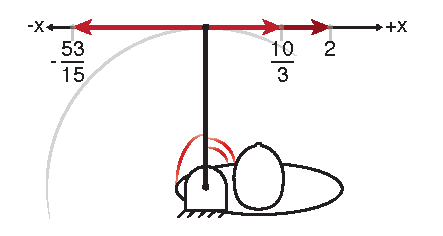
\includegraphics[width=0.5\textwidth]{figs/schematic_arm_1D.pdf}
  \caption{One imagined visualization of the fabricated tendon driven system, with 3 generators.}
  \label{fig:finger}
\end{figure}


\begin{figure}[ht]
  \label{fig:fig_hr}
   \begin{center}
    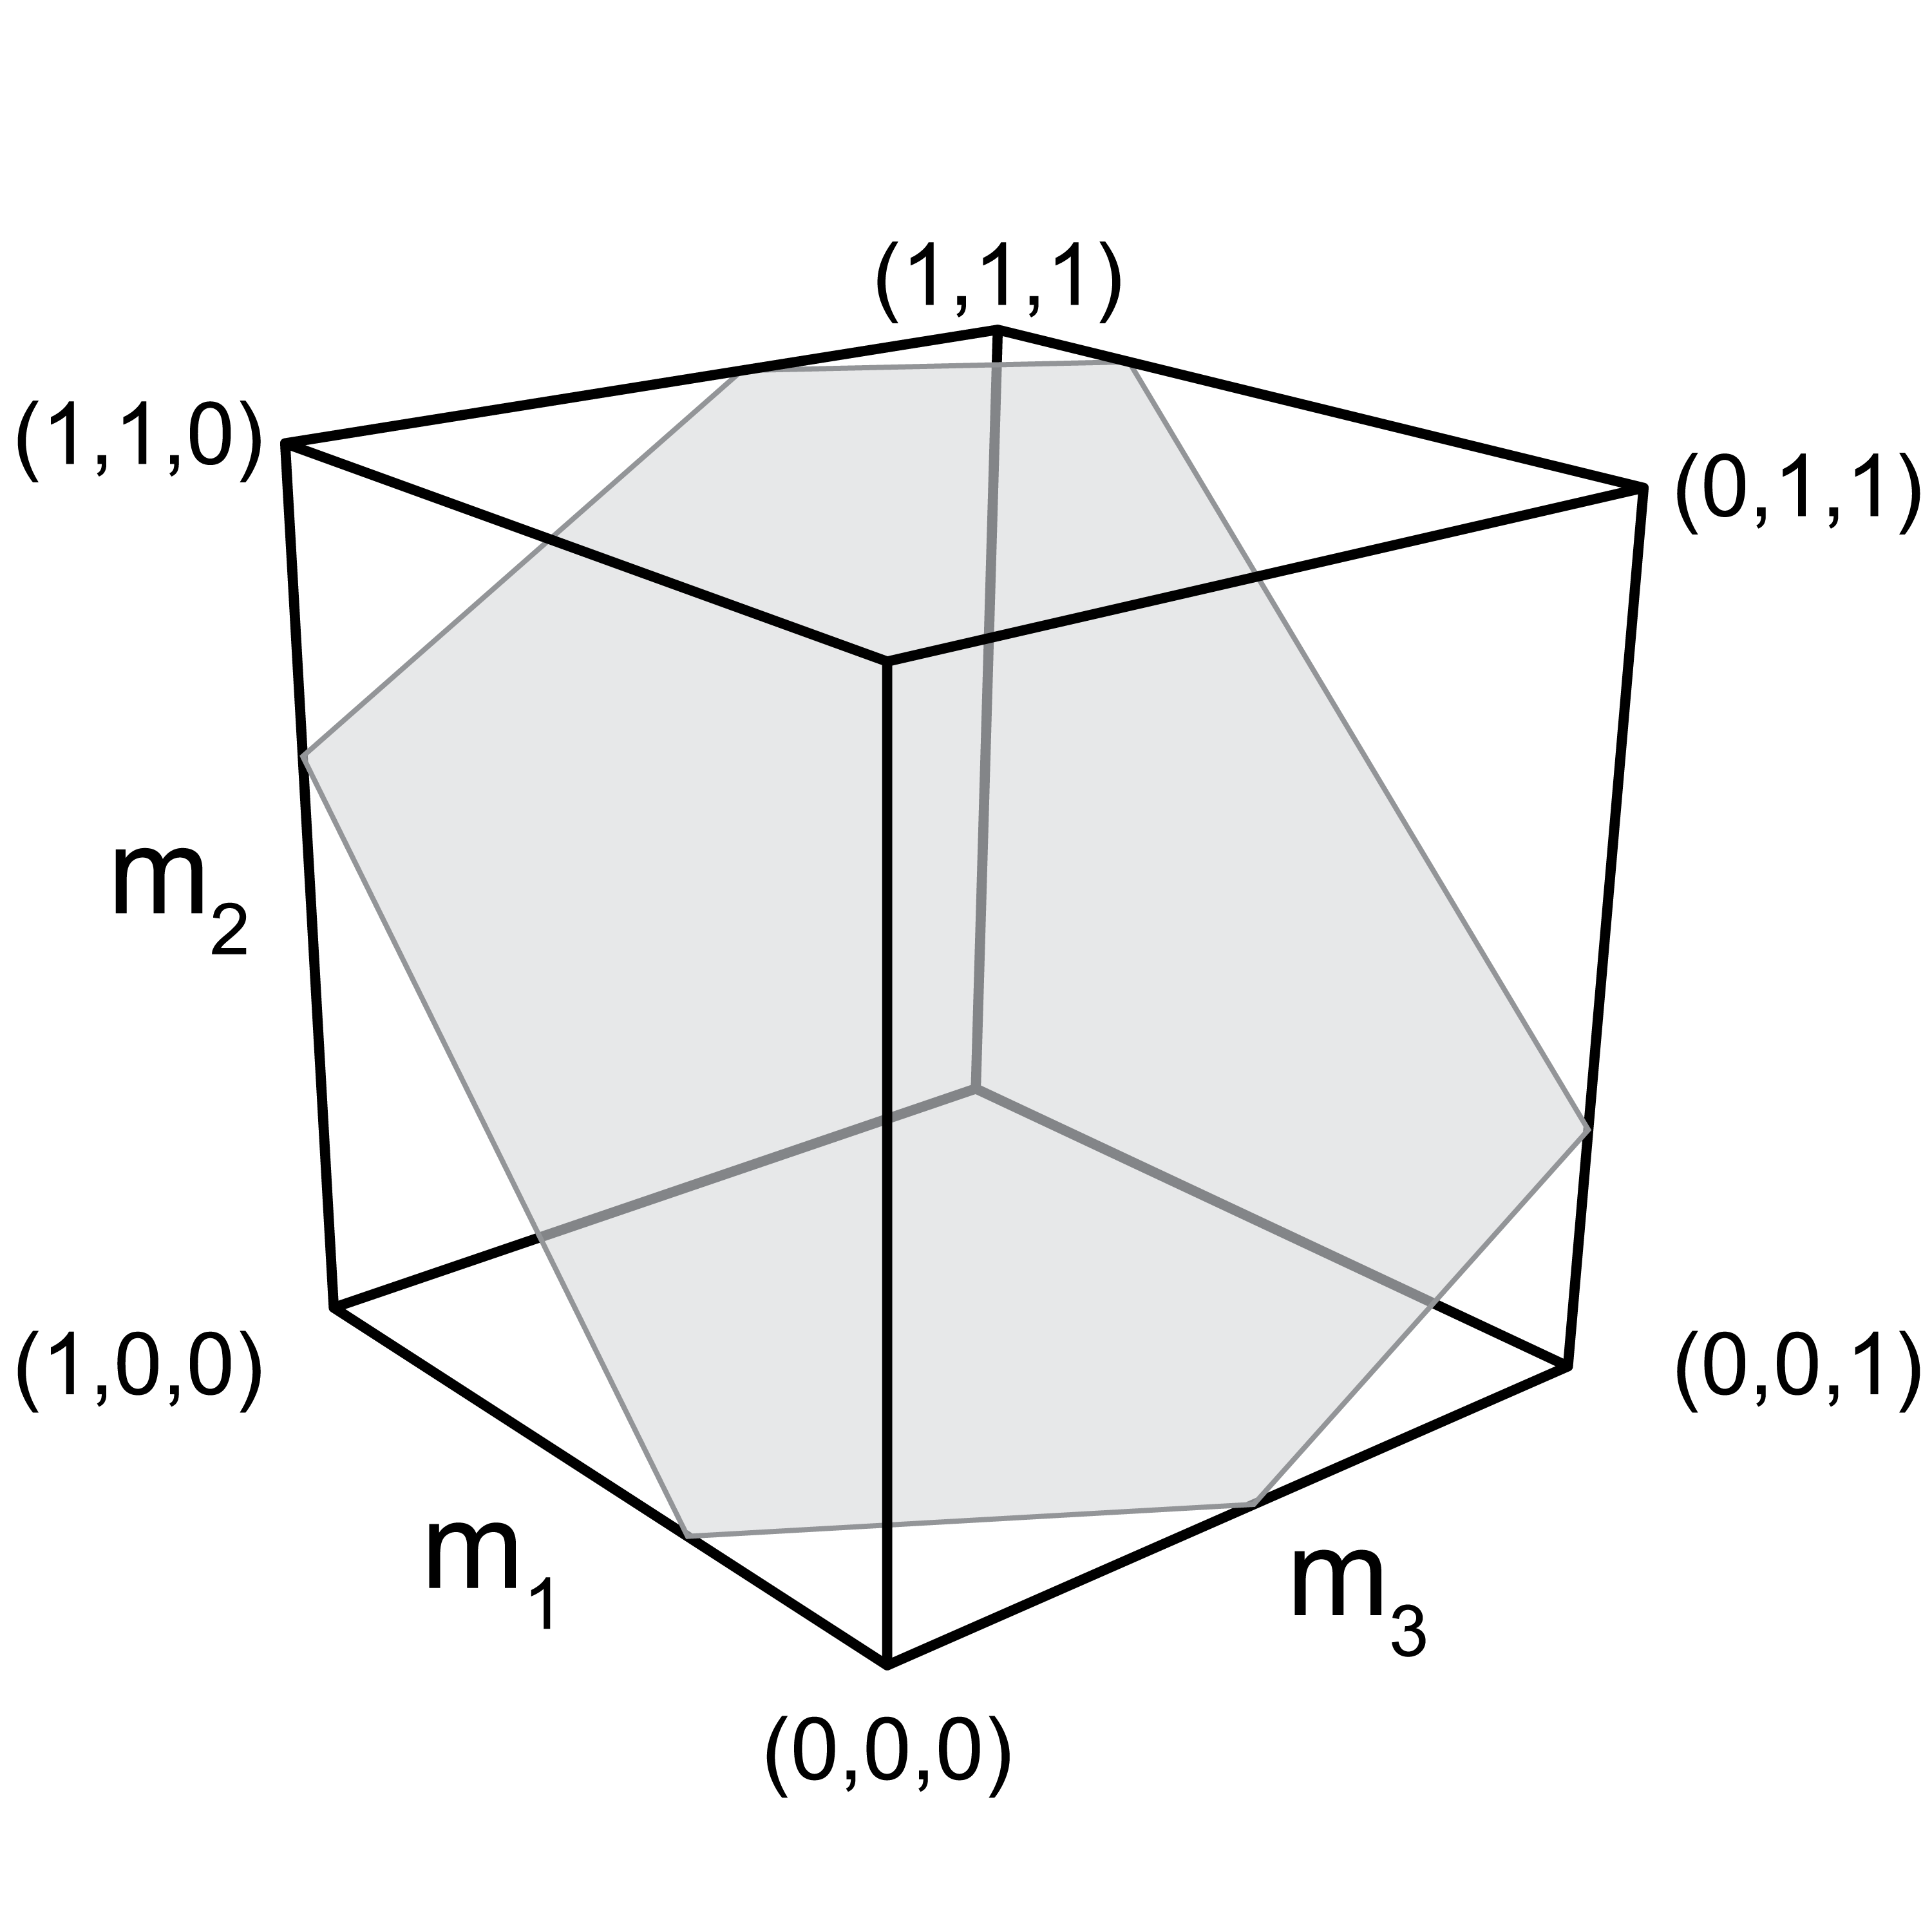
\includegraphics[width=0.25\textwidth]{sections/figs/feasibleactivation.png}
  \end{center}
  \caption{The feasible activation set for a  three-muscle system meeting one functional constraint is a polygon in $\mathbb{R}^3$.} %Note that muscle activations are assumed to be bounded between $0$ and $1$.}
\end{figure}

\subsection{Difficultis of Volume Computation in Higher Dimension}

Exact volume computations for polytopes is know to be $\#P$-hard \cite{Dyer}. Several algorithms have been suveyed and implemented, but can only handle up to 10 dimensions \cite{Bueler2}.  
%We aimed to compare the relative volumes of different sections of the activation space; however, exact volume computations are computationally intractable in dimensions beyond [maytodo cite]. 
Recent muscle system models we have used have been 31 dimensional \cite{Valero-Cuevas2015high-dimensional}, and other muscle models have over 40 muscles involved \cite{arnold2010model, kutch2012challenges, hamner2010muscle, de2014human}, thereby limiting the feasibility of using direct volume computations. Instead, we chose to uniformly sample the continuous space, effectively approximating the shape of the polytope by calculating point densities. %[maytodo mention whether the volume computation is a closed-form solution]

\subsection{Hit-and-Run algorithm}
\label{ss:hitrun}
We chose to sample the activation space with the Hit-and-Run method that is known to converge to the uniform distribution across an< convex body $K$ \cite{smith1984efficient}. It is a generalization of the discrete Markov chains and recursively samples a sequence of points in $K$ as described below. The mixing time is known to be $\mathcal{O}^*(n^2R^2/r^2)$, where $r$ and $R$ are the radii of the inscribed and cicumscribed ball of $K$ respectively \cite{Dyer, Lovasz}. I.e., after $\mathcal{O}^*(n^2R^2/r^2)$ steps, the Hit-and-Run algorithm has sampled a point uniformly at random (u.a.r.) in $K$. Unfortunately the hidden constant is large, which makes the problem practically almost infeasible. However experimental results suggest that a number of points linear w.r.t.\ to the dimension suffices; this will be discussed in Section \ref{sec_lengthrun}.
As the feasible activation space of the muscles are given by a convex polytope, this method can be directly applied for our problem. Notably, there are other methods which sample uniformly, such as the Grid Walk or Ball walk \cite{Vempala}. We chose the Hit-and Run because of its easy structure and mixing guarantee, however it would be interesting to compare with other methods.

The Hit-and-Run walk on $P$ is defined as follows (it works analogously for any convex body):
\begin{enumerate}
\item Find a starting point $\textbf{p}$ of $P$. %(Figure \ref{fig:hitruncube}a) .
\item Generate a random direction from $\textbf{p}$ in $P$ (uniformly at random over all directions) (Figure \ref{fig:hitruncube}a).
\item Find the intersection points of the random direction with the boundary of the polytope (Figure \ref{fig:hitruncube}b).
\item Choose a point u.a.r.\ on this line segment given by the intersection points (Figure \ref{fig:hitruncube}c). 
\item Repeat from $1.$ the above steps with the new point as the starting point .
\end{enumerate}

\begin{figure}[h]
\centering
\includegraphics[width=0.5\textwidth,page=10]{sections/figs/HitandRunSchematics_all.pdf}
\caption{Graphical description of the Hit-and-Run algorithm.}
\label{fig:hitruncube}
\end{figure}

\begin{figure}[h]
\centering
\includegraphics[width=0.3\textwidth,page=9]{sections/figs/HitandRunSchematics_all.pdf}
\caption{Uniform distribution aross the feasible activation space. In the schematic arm example, the distribution is represented within a 2D plane.}
\label{fig:posthitrun_distribution}
\end{figure}

\subsection{Implementation of Hit-and-Run}
To find a starting point in $P$ the polytope given by
\[\textbf{f} = A\textbf{a}, \textbf{a} \in [0,1]^n,\]
we only need to find a feasible activation vector. For the Hit-and-Run algorithm to mix faster we want the starting point not close to a vertex of the polytope \cite{Lovasz}. %centrally located point within the polytope- that way, the early points will not be clustered in a corner [maytodo cite]. 
We use the following standard trick with slack variables $\epsilon_i$, which for applications often gives a good starting point.% to select a point where activations $a_i$ for all muscles are far from 0 and 1, thereby finding a solution central within $P$ [maytodo cite the use of slack variables to improve mixing time].

\begin{equation}\label{eq:LP_r}
\begin{array}{lrcl}
\mbox{maximize} & \sum_{i=1}^n \epsilon_i \\ 
\mbox{subject to} & \textbf{f} &=& A\textbf{a}\\
  & a_i &\in& [\epsilon_i, 1- \epsilon_i], \hspace{5mm} \forall i \in \{1,\dots,n\}  \\
  & \epsilon_i &\geq& 0, \hspace{5mm} \forall i \in \{1,\dots,n\}.  
\end{array}
\end{equation}


The rest of the implementation of the Hit-and-Run algorithm is straight forward except for the choice of the random direction. How do we sample u.a.r.\ from all directions in $P$? Suppose that $\textbf{q}$ is a direction in $P$ and $\textbf{p} \in P$. Then by definition of $P$, $\textbf{q}$ must satisfy $\textbf{f} = A(\textbf{p}+\textbf{q})$. Since $\textbf{p} \in P$, we know that $\textbf{f} = A\textbf{p}$ and therefore 
\[\textbf{f} = A(\textbf{p} + \textbf{q}) = \textbf{f} + A\textbf{q} \Rightarrow A\textbf{q} = 0. \]
%and hence
%\[A\textbf{q} = 0.\]

and hence need to choose directions uniformly at random from all directions in the vectorspace 
\[V = \{\textbf{q} \in \mathbb{R}^n | A\textbf{q} = 0\}.\]

As shown by Marsaglia this can be done as follows \cite{Marsaglia}.

\begin{enumerate}
\item
Find an orthonormal basis $b_1, \dots, b_r \in \mathbb{R}^{n}$ of $A\textbf{q} =0$.
\item
Choose $(\lambda_1, \dots, \lambda_r) \in \mathcal{N}(0,1)^r$ (from the Gaussian distribution).
\item
$\sum_{i=1}^r \lambda_i b_i$ is a u.a.r.\ direction.
\end{enumerate}

A basis of a vectorspace $V$ is a minimal set of vectors that generate $V$, and it is orthonormal if the vectors are pairwise orthogonal (perpendicular) and have unit length. Using basic linear algebra one can find a basis for $\{A\textbf{q} = 0\}$ and orthogonalize with the well known Gram-Schmidt method (for details see e.g.\ \cite{Robertson}). Note that in order to get the desired u.a.r.\ sample the basis needs to be orthonormal. For the limb case we can safely assume that the rows of $A$ are linearly independent and hence the number of basis vectors is $n-m = r$.

\subsection{Mixing Time}
\label{sec_lengthrun}
From a given starting point, how many iterations of the Hit-and-Run method are necessary to reach a u.a.r.\ point? For convex polygons in higher dimensions up to $40$, experimental results suggest that $\mathcal{O}(n)$ steps of the Hit-and-Run algorithm are sufficient.
In particular Emiris and Fisikopoulos paper suggest that $(10 + \frac{10}{n})n$ steps are enough to converge upon the uniform distribution \cite{emiris2013efficient}, while in Ge et al.'s paper every point of the Hit-and-Run algorithm is used in the sample \cite{Ge}. 

\subsection{Realistic index finger model}
\label{ss:finger}
We used our published model in \cite{Valero-Cuevas1998Large} to find matrix $A \in \mathbb{R}^{4 \times 7}$, where $\textbf{a} \in \mathbb{R}^7$; the four degrees of freedom were ad-abduction, flexion-extension at the metacarpophalangeal joint, and flexion-extension at the proximal and distal interphalangeal joints.
The force direction we simulated are visible in Figure \ref{fig:finger}.
In this model, for each input we collected 1.000.000 points and sampled every 100th point.
In addition to the Hit-and-Run algorithm we computed the theoretical maximum and minimum activation for each muscle for the given force; the difference between the theoretical and observed bounds for all muscles is smaller than 0.001. \ref{fig:raw_histograms, fig:Z_progression}.

\begin{figure}[htbp]
  \centering
  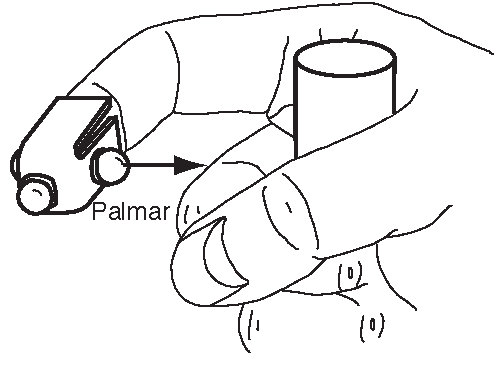
\includegraphics[width=0.5\textwidth]{sections/figs/finger.pdf}
  \caption{The index finger model simulated force production in the palmar direction. Adapted from \cite{Valero-Cuevas1998Large}.}
  \label{fig:finger}
\end{figure}

\subsection{Solution projection histograms}
Figure \ref{fig:raw_histograms} shows the activation distribution of each muscle, when activated with $50\%$ of the maximal activation force. We also show the observed activation upper and lower bounds for each muscle (vertical dotted lines).
In Section \ref{sub:activation_spaces_for_increasing_force} we consider the distributions for different forces into palmar direction.
\begin{figure}[!htbp]
\centering
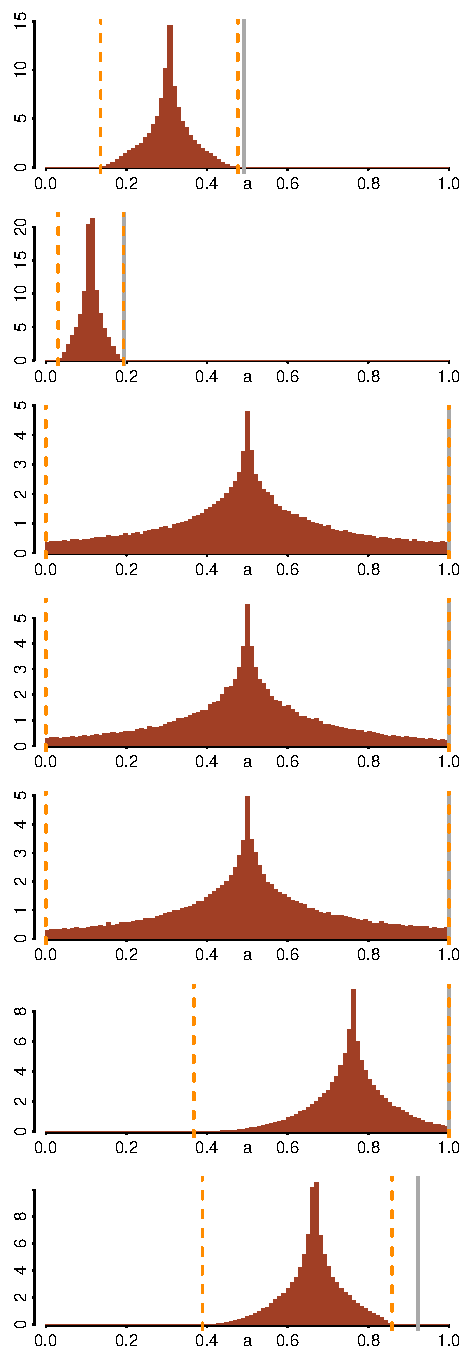
\includegraphics[width=0.5\textwidth]{figs/raw_histograms.pdf}
\caption{Distribution of feasible activations for 50\% of the computed maximal force output in the palmar direction.}
\label{fig:raw_histograms}
\end{figure}

\subsection{Parallel coordinates visualization}
A common way to visualize higher dimensional data is using parallel coordinates[briantodo citations]. To show our sample set of points in the feasible activation space we draw $n$ parallel lines for each of the $n$ muscles.
With the axis labels of the line set between 0 and 1, each point is then represented by connecting their coordinates by $n-1$ lines.
Using an interactive surface we restrict each muscle function to any desired interval- see Figures \ref{fig:parcoord_full} and \ref{fig:parcoords}.
We decided to simulate a 50\% reduction in activation (feasible tendon force production) in three of the muscles innervated by the deep branch of the ulnar nerve- PI, DI, and FDP. 

\subsection{Muscle-metabolic and neural drive cost functions}

For every solution collected, we used popularly-used cost functions: we computed activation $l_1$, $l_2$ and $l_3$ norms, and the tendon-force $l_1^w$, $l_2^w$ and $l_3^w$ norms.


\begin{table}[h]
\centering
\begin{tabular}{@{}ll@{}}
\toprule
\textbf{Name} & \textbf{Cost function}  \\ \midrule
$l_1$            & $\sum_{i=1}^n a_i$                                     \\
$l_2$            & $\sqrt{\sum_{i=1}^n a_i^2}$                                    \\
$l_3$            & $\sqrt[3]{\sum_{i=1}^n a_i^3}$                                   \\
$l_1^w$            & $\sum_{i=1}^n a_i F_{0i}$                                    \\
$l_2^w$            & $\sqrt{\sum_{i=1}^n (a_i F_{0i})^2}$                                  \\
$l_3^w$            & $\sqrt[3]{\sum_{i=1}^n (a_i F_{0i})^3}$                                    \\ \bottomrule
\end{tabular}
\caption{Cost functions and their usage, where $a_i$ and $F_{0i}$ represent a muscle's activation in a given solution and that muscles MIC [briantodo: what is MIC?], respectively.}
\label{cost_function_tabls}
\end{table}

Six additional vertical lines were added to the parallel coordinates plot to represent each cost function. With the same parallel coordinates framework as developed with muscle activation, we can restrict and subset solutions which fall into desired cost-function ranges, thereby masking sub-optimal solutions and highlighting only those meeting the criteria.
For a given point $\textbf{a} \in \mathbb{R}^n$ we are interested in the associated cost of every solution collected through Hit-and-Run.
We developed and tested our code in  Ubuntu 14.04, Windows 8.1, and OSX Yosemite, using Scala 2.11.6 [briantodo cite] for our implementation of Hit-and-Run, R 3.1.3 [briantodo cite] for histograms and plots, and using Sygmatic Parcoord[briantodo cite] and d3.js[briantodo cite] for our interactive parallel coordinate visualization. All code used to develop this publication is readily available at https://github.com/bcohn12/space.
\begin{figure}[htbp]
\centering
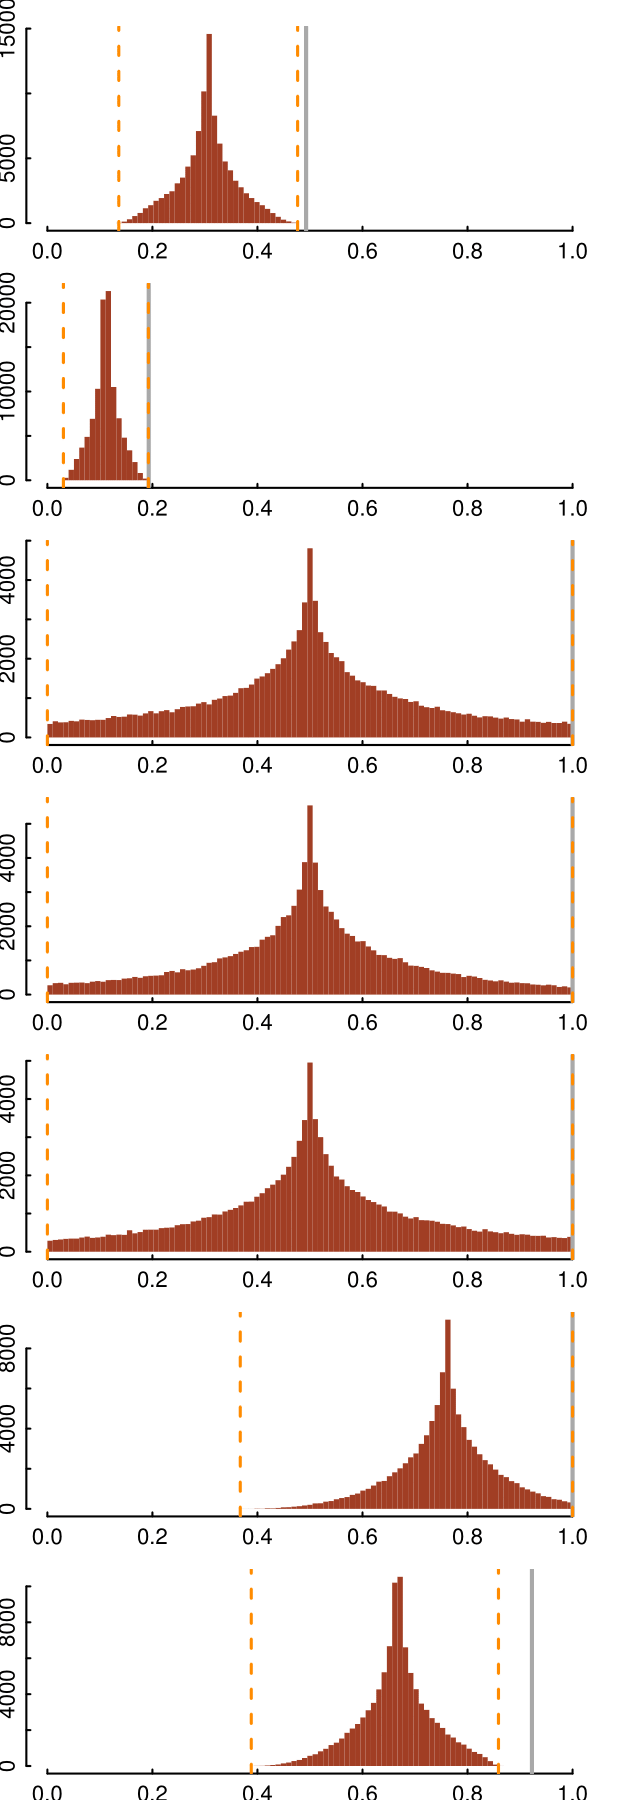
\includegraphics{sections/figs/raw_histograms.png}
\caption{Distribution of feasible activations for 50\% maximal force output in the palmar direction.}
\label{fig:raw_histograms}
\end{figure}


briantodo: add the following figures:
\begin{itemize}
\item{parcoord Full}
\item{parcoord muscle limited to 75\percent, then 50\percent, then 25\percent}
\item{}


\section{RESULTS}

Using Hit-and-Run to sample feasible activation sets, Figure \ref{fig:raw_histograms} shows the distributions of activation solutions for a palmar submaximal force.resulting from $1,000,000$ solutions computed with Hit-and-Run sampling. This is the first time (to our knowledge) that the internal structure of the feasible activation set has been visualized for a sub-maximal force.

Notice also that the lower and upper bounds of the activations (i.e., the dashed lines that indicate their bounding box), are uniquely uninformative of the actual density of distribution of feasible activations. Note also that the activation needed for the maximal force output (thick gray line) is very often not the mode of the activations at 50\% of output.


Results:
Projection onto a given muscle dimension
Simple histograms at 80% activation for one direction
Activation progression-march (3) x y z
Parallel coordinates with cost
	Full
Parallel Coordinates with cost
	Lower
	Middle
	Upper
	constraint by cost
		Yes you could put activation constraints directly in the A matrix, instead of bounds between 0 and 1. There is no advantage to adding activation constraints beforehand in the A matrix, as sampling is uniform- as long as the resulting dataset is large enough for your purpose.
		You could also put l1 and weighted l1 cost bounds as constraints in the A matrix. Cannot put higher order cost functions such as l2,l3 or weighted l2,l3.

		Talk about slopes in Parallel
		if they 


\section{DISCUSSION}

\subsection{Level of trust of the polytope approximation} % (fold)
\label{sub:level_of_trust_of_the_polytope_approximation}

Our approximations show sufficiently accurate views of the polytope in slices perpendicular to each axis. Had we performed exact volume computations, we would have had more accurate relative volumes; that said, the level of error generated through approximation is exceptionally small in comparison to error derived from measuring/predicting the musculoskeletal parameters to define the force generators $A$. Our code only solves one linear equation to find the starting point, and the time-cost of each point thereafter is linear; therefore this method can be used for tendon driven models in very high-dimensional systems.

Sohn et. al. have identified how the bounding box can illustrate the bounds of feasible activation; essentially reducing the effective number of solutions a neuromuscular system can select from \cite{sohn2013cat_bounding_box}. Our research here looks to further constrain this space by observing the cost-agnostic distribution of solutions across the set of all feasible coordination patterns.

% subsection level_of_trust_of_the_polytope_approximation (end)
\subsection{Activation Progression} % (fold)
\label{sub:activation_progression}
The only way that the bounding box would contain the entire set of information regarding a given muscle's activation distribution would be if that end effector is completely unaffected by any activation of that muscle i.e. the muscle's linear endpoint force is the 0 vector. As such, muscles which are nearly uninvolved in the end effector's actions will form near-uniform distributions, as their involvement does not affect the activation space.
% subsection activation_progression (end)

\subsection{Features of the PDF} % (fold)
\label{sub:features_of_the_pdf}
why must they be \\
unimodal\\
non-normal\\
non-uniform (talk about the exception(s))\\
what the exact pdf function would be \\
	a piecewise quadratic equation, where it changes when you incorporate/exclude vertices of the polytope
% subsection features_of_the_pdf (end)

\subsection{Parallel coordinate slopes} % (fold)
\label{sec:parallel_coordinate_slopes}
[maytodo: Talk about what it means to have slopes in Parallel, what a very positive slope means/what a very negative slope means, and what the crossing-slopes mean. Also put forward a couple suggestions of how these slopes could be more quantitatively interpreted/analyzed]
% subsection parallel_coordinate_slopes (end)

\subsection{Cost distributions} % (fold)
\label{sec:cost_distributions}
In further studies one could put activaton constraints directly into the $A$, instead of the unit interval bounds. As long as the resulting dataset is large enough for our purpose, there is no advantage to this, as we can not compare with the original feasible activation space. Since $l_1$ and $l_1^w$ are linear, one can also put corresponding constraints into $A$. Our implementation does not support directily inputting bounds on the higher degree weight functions $l_2$, $l_3$, $l_2^w$ and $l_3^w$.
%Yes in further studies we could put activation constraints directly in the A matrix, instead of bounds between 0 and 1. But there are no advantages to adding activation constraints beforehand in the A matrix, as sampling is uniform- as long as the resulting dataset is large enough for your purpose.
%You could also put l1 and weighted l1 cost bounds as constraints in the A matrix. Cannot put higher order cost functions such as l2,l3 or weighted l2,l3.

We note that the activation and metabolic classes of cost function are fundamentally different, and do not explore correlations between these two classes. We do, however, note that when all of the involved cost functions are 'minimized' to the bottom half of all solution costs, the union maintains a very high number of solutions (22\%). With this we can note how all of these cost functions are similar in nature across the polytope (as expected).
% subsection cost_distributions (end)

\subsection{Concluding remarks} % (fold)
\label{ssub:concluding_remarks}

Our results clearly show:
\begin{itemize}
	\item{The Hit-and-Run algorithm can explore the feasible activation space for a realistic 7-muscle finger in a way that is computationally tractable.}
	\item{We find that the bounding box exceptionally misconstrues the internal structure of the feasible activation set.}
	\item{The Hit-and-Run algorithm is cost-agnostic in the sense that no cost function is needed to predict the distribution of muscle activation patterns. Therefore, we can provide spatial context to where 'optimal' solutions lie within the solution space; this approach can be used to explore the consequences of different cost functions.}
	\item{The distribution of muscle activations often show and strong modes that will critically affect the learning of motor tasks.}
\end{itemize}
In comparison to traditional bounding-box representations, our application of Hit-and-Run in this context is decisively superior in capability for meaningful visualization, value in extracting associations between solutions, and computational tractability, in addition to being veritable of the true solution distributions within the feasible activation set. Our bodies exist within a feasible activation space, and once we enter this space then optimization is possible. In this way, we can think of the solutions space as an effectie model for exporation-exploitation.
This can help us in comparing the structure of the activation space as a set of high-dimensional bayesian priors which are narrowed/shifted over time to compensate for learning and skill-development.
Essentially, once you enter into task-independent variation, it becomes a question of identifying the region of the activaiton space which both satisfieds the spatiotemporal constraints, but also approaches optimality under efficiency/speed demands.
We want to 'close the loop' between the nervous system commands, and the mechanical output, thereby uncovering how the CNS collaborates with newtonian physics to select neural commands which effecitvey coordinate multi-link limbs, so we can act, play, and dance in the real world.
Mechanical demands constrain the total space of musculoskeletal coordination options, thus, motile organisms first 'explore' coordination strategies conducive to the desired movement, and recursively redefine the more optimal subspaces.
Once a desired task is mapped to an effective coordination strategy (as in, it gets the job done), then training and experience (exploration-exploitation) can aid in finding the best coordination.
As many tasks are similar (ie. they require the similar force generation or torque production over the course of a movement),  the activation patterns for simlar actions must be similar as well.
Optimal coordination strategies for one task may be near-optimal for a similar task.
On the other hand, a suboptimal coordination strategy that achieves one task, may be furiously off-target for a very similar task.

intention --> excitation --> activation dynamics --> contraction properties --> muscle properties with muscle models --> musculoskeletal force on the bones, joints, and finally, endpoint force. Long chain and we only look at 2 parts.

[briantodo: discuss francisco's paper about scaling the solution to the boundary.]

% subsubsection concluding_remarks (end)

[briantodo: address the following:]
any given manuscript must satisfy the following criteria:
\begin{itemize}
	\item {Originality}
	\item {Innovation}
	\item {High importance to researchers in the field}
	\item {Significant biological and/or methodological insight}
	\item {Rigorous methodology}
	\item {Substantial evidence for its conclusions}
\end{itemize}












  

\addtolength{\textheight}{-12cm}   % This command serves to balance the column lengths
                                  % on the last page of the document manually. It shortens
                                  % the textheight of the last page by a suitable amount.
                                  % This command does not take effect until the next page
                                  % so it should come on the page before the last. Make
                                  % sure that you do not shorten the textheight too much.

%%%%%%%%%%%%%%%%%%%%%%%%%%%%%%%%%%%%%%%%%%%%%%%%%%%%%%%%%%%%%%%%%%%%%%%%%%%%%%%%



%%%%%%%%%%%%%%%%%%%%%%%%%%%%%%%%%%%%%%%%%%%%%%%%%%%%%%%%%%%%%%%%%%%%%%%%%%%%%%%%



%%%%%%%%%%%%%%%%%%%%%%%%%%%%%%%%%%%%%%%%%%%%%%%%%%%%%%%%%%%%%%%%%%%%%%%%%%%%%%%%


%%%%%%%%%%%%%%%%%%%%%%%%%%%%%%%%%%%%%%%%%%%%%%%%%%%%%%%%%%%%%%%%%%%%%%%%%%%%%%%%


\bibliographystyle{plain}
\bibliography{sections/ieee}


\end{document}
